\documentclass[a4paper,11pt]{article}
\input{/home/tof/Documents/Cozy/latex-include/preambule_lua.tex}
\newcommand{\showprof}{show them}  % comment this line if you don't want to see todo environment
\fancyhead[L]{Interaction côté client}
\newdate{madate}{10}{09}{2020}
%\fancyhead[R]{\displaydate{madate}} %\today
%\fancyhead[R]{Seconde - SNT}
\fancyhead[R]{Première - NSI}
%\fancyhead[R]{Terminale - NSI}
\fancyfoot[L]{~\\Christophe Viroulaud}
\AtEndDocument{\label{lastpage}}
\fancyfoot[C]{\textbf{Page \thepage/\pageref{lastpage}}}
\fancyfoot[R]{\includegraphics[width=2cm,align=t]{/home/tof/Documents/Cozy/latex-include/cc.png}}

\begin{document}
\begin{Form}
\begin{commentprof}
fichier site-specialites.zip sur site
\end{commentprof}
\section{Problématique}
Dans un souci de rendre \emph{la page de présentation des spécialités} plus attrayante pour les visiteurs, on se propose d'apporter de l'interactivité dans le contenu. En effet, cette \emph{page statique} ne propose pour l'instant que des liens vers des pages web externes. Par exemple, il pourrait être intéressant d'afficher sur la même page, divers contenus en fonction des clics.
\begin{figure}[!h]
\centering
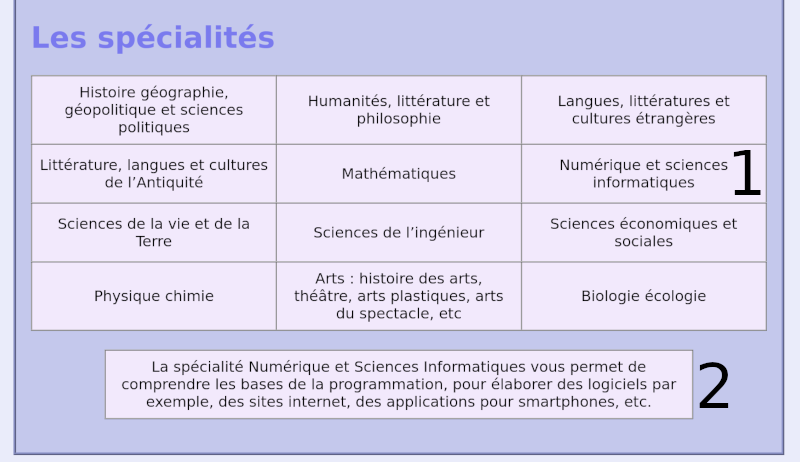
\includegraphics[width=10cm]{ressources/problematique-legende.png}
\captionof{figure}{En cliquant dans la cellule \textbf{1} la description de la spécialité apparaît dans la cellule \textbf{2}.}
\label{IMG}
\end{figure}
\begin{center}
\shadowbox{\parbox{10cm}{\centering Comment modifier une page web de manière interactive?}}
\end{center}
\section{Requête http}
\subsection{Principe général}
\textbf{HTTP (HyperText Transfer Protocol)} est un protocole élaboré par Tim Berners-Lee en même temps que le système d'adresse \emph{URL (Uniform Ressource Locator)} et le langage \emph{HTML (HyperText Markup Language)}, pour créer le \emph{World Wide Web}.
\begin{aretenir}[]
Ce protocole permet de récupérer des ressources telles que des documents HTML. Il est à la base de tout échange de données sur le Web. C'est un protocole de type \emph{client-serveur} (figure \ref{http}), ce qui signifie que les requêtes sont initiées par le destinataire (qui est généralement un navigateur web).
\begin{flushright}
\scriptsize{Mozilla Developpement Network}
\end{flushright}
\end{aretenir}
\begin{center}
\centering
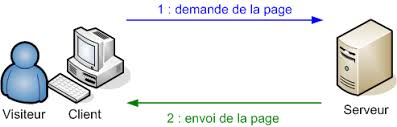
\includegraphics[width=8cm]{ressources/http.jpeg}
\captionof{figure}{Protocole HTTP}
\label{http}
\end{center}
\subsection{Détails des requêtes}
En premier approche nous pouvons considérer que la requête s'effectue en deux étapes:
\begin{itemize}
\item Requête \begin{center}
\centering
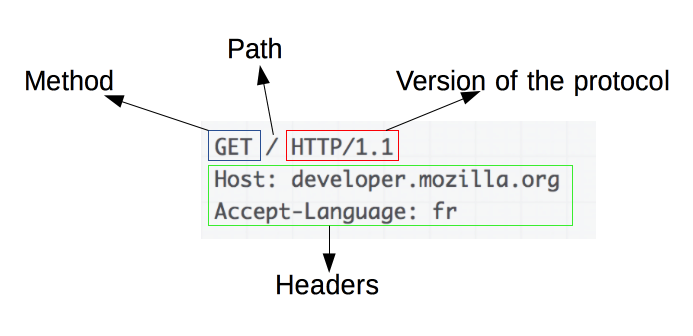
\includegraphics[width=7cm]{ressources/HTTP_Request.png}
\captionof{figure}{Le client (le navigateur) demande la page web au serveur.}
\label{demande}
\end{center}
\item Réponse \begin{center}
\centering
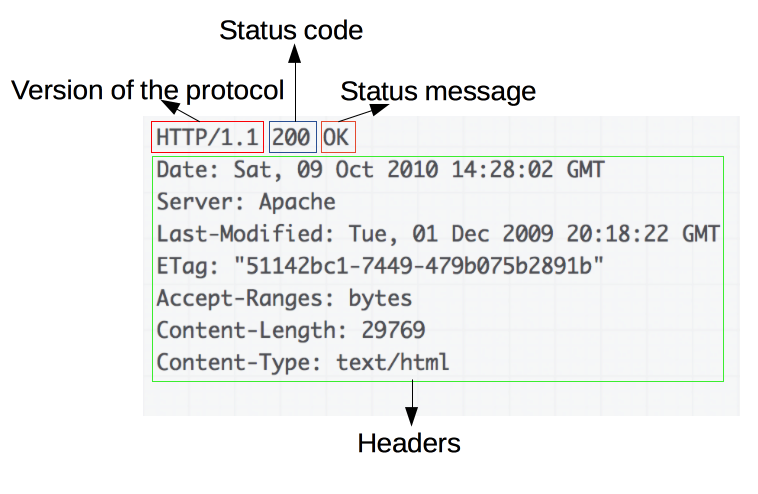
\includegraphics[width=7cm]{ressources/HTTP_Response.png}
\captionof{figure}{Le serveur renvoie la page demandée.}
\label{demande}
\end{center}
\end{itemize}
\begin{activite} L'objectif est de retrouver les requêtes effectuées. Selon le navigateur utilisé la méthodologie est sensiblement différente
\begin{enumerate}
\item \textbf{Sur Firefox:}
\begin{enumerate}
\item  Cliquer sur \emph{Ctrl+Shift+E}, le panneau \emph{réseau} s'ouvre.
\item Ouvrir la page \mbox{\url{http://jay.info.free.fr}}
\item Ouvrir la ligne \emph{GET}.
\begin{center}
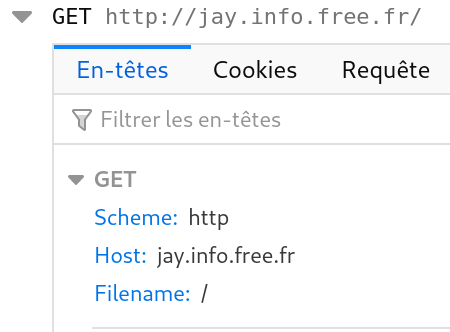
\includegraphics[width=6cm]{ressources/requete-ff.png}
\end{center}
\item Dans \emph{En-têtes}, retrouver alors les informations transmises et retournées.
\end{enumerate}
\item \textbf{Sur Chrome:}
\begin{enumerate}
\item  Cliquer sur \emph{Ctrl+Shift+I}, un panneau s'ouvre.
\item Choisir \emph{Réseau} ou \emph{Network}.
\item Ouvrir la page \mbox{\url{http://jay.info.free.fr}}
\item Cliquer sur \emph{jay.info.free.fr}.
\begin{center}
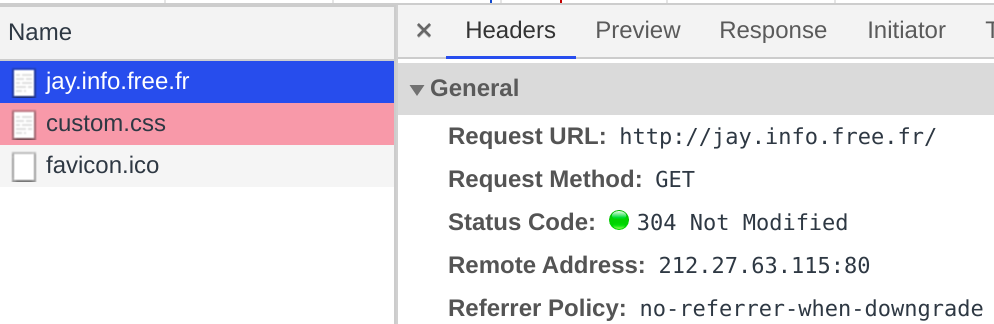
\includegraphics[width=6.5cm]{ressources/requete-chrome.png}
\end{center}
\item Dans \emph{Headers}, retrouver alors les informations transmises et retournées.
\end{enumerate}
\item Quelle est la version du protocole \emph{HTTP} utilisé?
\item Quelle est la dernière date de modification de la page?
\item Exécuter les mêmes opérations avec un site plus évolué:  \mbox{\url{https://cviroulaud.github.io}}
\item Combien de requêtes \emph{GET} le navigateur a-t-il effectué pour charger la page?
\end{enumerate}
\begin{aretenir}[]
Une page web moderne contient de nombreux contenus stockés sur différents serveurs (texte, image, vidéo, bibliothèque...). Le navigateur effectue plusieurs requêtes pour récupérer ces données puis construire l'affichage de la page.
\end{aretenir}
\end{activite}
\section{JavaScript}
\subsection{Contexte historique}
C'est un langage de programmation de \emph{scripts} c'est à dire qui permet de manipuler les fonctionnalités d'un système informatique. Il a été crée en mai 1995 par \emph{Brendan Eich} pour le compte de la Netscape Communications Corporation.
\subsection{Le DOM}
Le \textbf{DOM (Document Object Model)} est une interface qui permet de manipuler le contenu des pages web. 
\begin{figure}[!h]
\centering
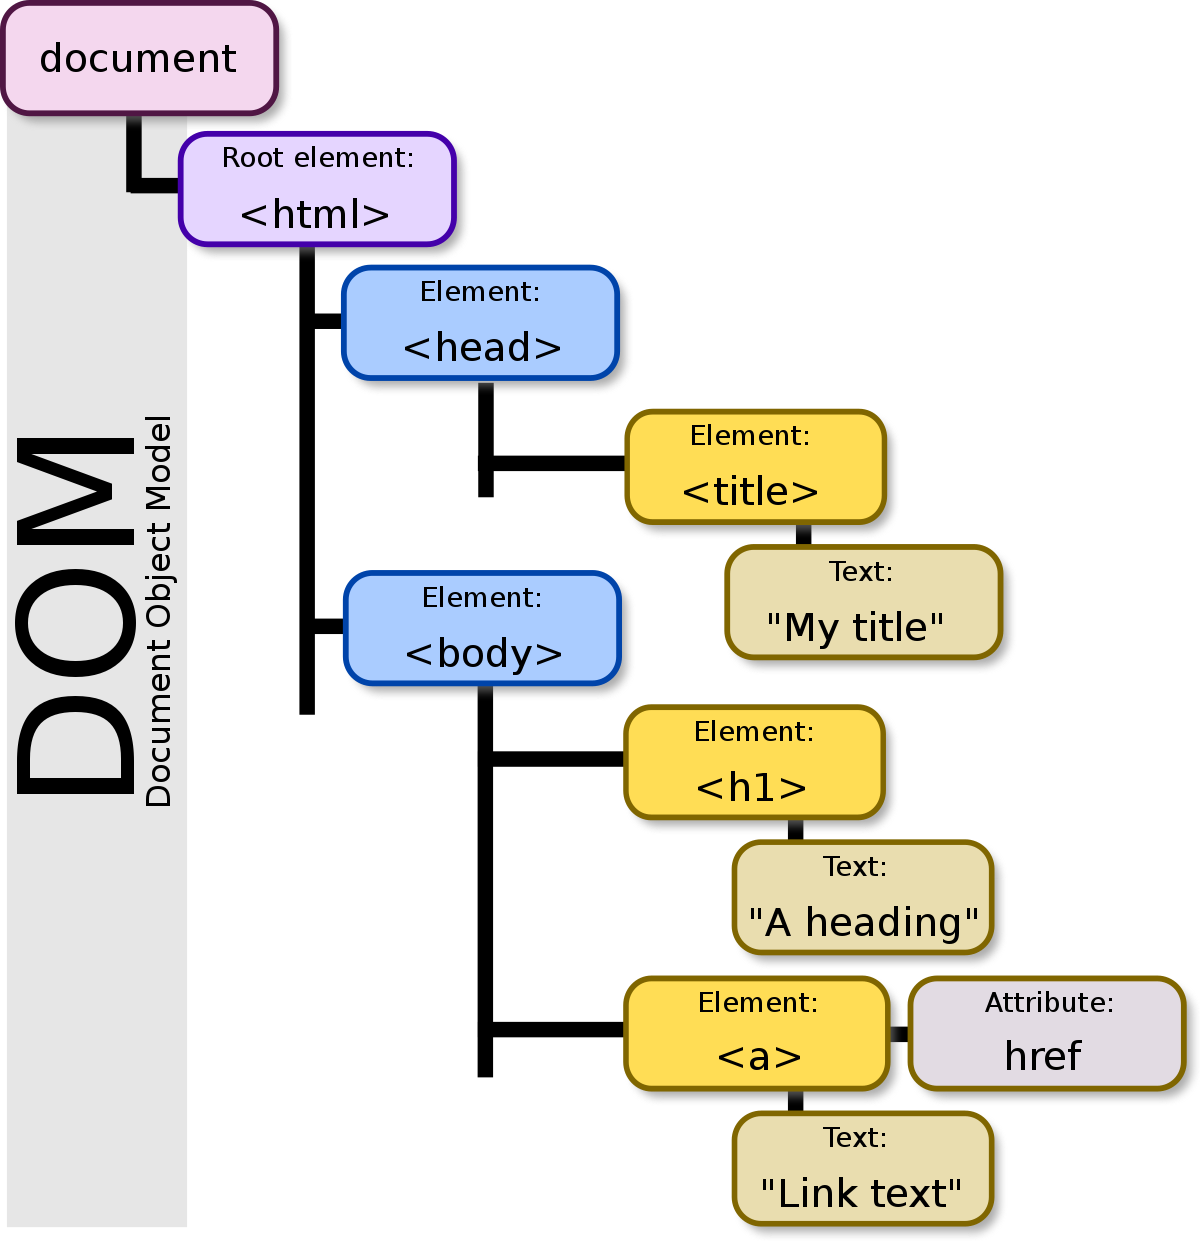
\includegraphics[width=6cm]{ressources/dom.png}
\captionof{figure}{Document Object Model}
\label{dom}
\end{figure}

On le nomme \emph{arborescence de nœuds (node tree)} (figure \ref{dom}) car il peut être considéré comme un arbre qui se ramifie en plusieurs branches enfants, chacune pouvant avoir des feuilles.
\begin{itemize}
\item Le premier parent est l'élément \emph{racine HTML}.
\item Un élément peut posséder des attributs et/ou du texte.
\begin{center}
\begin{lstlisting}[language=HTML]
<a href="https://cviroulaud.github.io">Super site</a>
\end{lstlisting}
\captionof{code}{Élément HTML}
\label{element}
\end{center}
Dans le  code \ref{element}:
\begin{itemize}
\item \emph{href} est un attribut,
\item \emph{Super site} est le texte affiché.
\end{itemize}
\end{itemize}
\subsection{Interagir avec le DOM}
Les éléments du DOM sont des objets atteignables grâce au JavaScript. Il existe plusieurs méthodes disponibles présentées en détails dans la documentation en ligne. Ces quelques références donnent un aperçu des possibilités:
\begin{itemize}
\item \url{https://tinyurl.com/ybuaoyuy}
\item \url{https://tinyurl.com/yxnyglbg}
\item et bien sûr le site de la MDN: \url{https://developer.mozilla.org/fr/docs/Web/API}
\end{itemize}
Concentrons-nous sur une méthode en particulier. L'élément \emph{a} du code HTML \ref{htmlid} possède un attribut \emph{id} (pour identifiant) et un attribut \emph{href}.
\begin{code}[!h]
\begin{lstlisting}[language=HTML]
<a id="monlien" href="http://monsite.fr">Un site web</a>
\end{lstlisting}
\captionof{code}{Code HTML}
\label{htmlid}
\end{code}

Le code JavaScript \ref{refjs} permet d'accéder à l'élément. Les lignes précédées de // sont des commentaires et ne sont pas exécutées.
\begin{code}[!h]
\begin{lstlisting}
// Le mot clé 'let' permet de déclarer une variable (nommée lien dans cet exemple)
let lien = document.getElementById("monlien");
\end{lstlisting}
\captionof{code}{Référencer un élément du DOM}
\label{refjs}
\end{code}
\begin{aretenir}[Remarque]
Le JavaScript est sensible à la casse. Il respecte le \emph{CamelCase}.\\
Il faut également remarquer le point-virgule en fin de chaque instruction.
\end{aretenir}

Le code \ref{modifjs} modifie le contenu de l'élément \emph{a} référencé  dans la variable \emph{lien}.

\begin{code}[!h]
\begin{lstlisting}
lien.textContent = "Le meilleur site web";
\end{lstlisting}
\captionof{code}{Modifier le texte d'un élément}
\label{modifjs}
\end{code}

Le code \ref{modifattr} modifie le lien référencé par l'attribut \emph{href}.
\begin{code}[!h]
\begin{lstlisting}
lien.setAttribute("href", "https://cviroulaud.github.io");
\end{lstlisting}
\captionof{code}{Modifier la valeur de l'attribut d'un élément}
\label{modifattr}
\end{code}

\begin{activite}
\begin{enumerate}
\item Créer une page HTML et placer l'élément \emph{a} du code \ref{htmlid}.
\item Juste avant la balise fermante </body>, placer le code \ref{scriptjs}.
\begin{center}
\begin{lstlisting}
<script src="main.js"></script>
</body>
\end{lstlisting}
\captionof{code}{Lier le code JavaScript au fichier HTML}
\label{scriptjs}
\end{center}
\item Créer un fichier \emph{main.js} dans le même dossier que le ficher HTML.
\item Copier les codes \ref{refjs}, \ref{modifjs} et \ref{modifattr} dans le fichier JavaScript.
\item Ouvrir le fichier HTML depuis un navigateur et vérifier que le lien a bien été modifié.
\item Depuis le navigateur, accéder au code source de la page.
\item Remarquer que le texte et les attributs du lien contiennent les valeurs codées dans le fichier HTML initial.
\end{enumerate}
\end{activite}
\subsection{Les écouteurs}
Grâce au JavaScript, il est possible de modifier le contenu de la page web lors de son chargement. L'étape suivante est de pouvoir interagir avec les actions de l'utilisateur.
\begin{aretenir}[]
Un  \textbf{écouteur d'événement} surveille les actions de l'utilisateur et exécute un code spécifique quand une de ces actions est réalisée.
\end{aretenir}

Les codes ci-après permettent de surveiller le clic sur un tableau HTML. 
\begin{center}
\begin{lstlisting}[language=HTML]
<table id="table-specialites">
\end{lstlisting}
\captionof{code}{Création d'un tableau dans la page HTML}
\label{moncode}
\end{center}

\begin{center}
\begin{lstlisting}[language=HTML]
let tabSpecialites = document.getElementById("table-specialites");
\end{lstlisting}
\captionof{code}{Référencement du tableau en JavaScript}
\label{moncode}
\end{center}
\begin{center}
\begin{lstlisting}
tabSpecialites.addEventListener('click', function(event) {
  //code exécuté lors du clic sur le tableau
  //ici une fenêtre 'bonjour' s'ouvre
  alert("bonjour');
});
\end{lstlisting}
\captionof{code}{Création de l'écouteur sur le tableau}
\label{moncode}
\end{center}

La documentation en ligne, notamment sur le site de la MDN \mbox{\url{https://tinyurl.com/n5zjs4u}} détaille davantage les spécificités des écouteurs.

\begin{activite}
\begin{enumerate}
\item Télécharger le fichier compressé \emph{site-specialites.zip} sur le site \mbox{\url{https://cviroulaud.github.io}}
\item Décompresser les fichiers et ouvrir le site depuis un navigateur.
\item Cliquer sur une cellule du tableau et observer la modification réalisée.
\item Depuis un IDE, observer le code du fichier \emph{main.js}.
\item Modifier les descriptions pour chaque spécialité en prenant modèle sur celle de la NSI.
\item Modifier le code pour qu'une image différente soit affichée pour chaque spécialité. Les images devront correspondre au thème de la spécialité.
\end{enumerate}
\end{activite}
\subsection{Exécution côté client}
Dans les exemple précédents, le code JavaScript est exécuté \emph{côté client}, c'est à dire par le navigateur. Deux indicateurs nous permettent de l'affirmer:
\begin{itemize}
\item Il n'y a pas de rechargement de la page lors d'un clic sur une cellule.
\item Le code source de la page HTML (accessible par un clic-droit) contient le code initial non modifié.
\end{itemize}
\begin{aretenir}[]
Le JavaScript modifie dynamiquement la page web. Le fichier HTML source n'est pas réécrit. Un rechargement de la page supprime les modifications réalisées par le code JavaScript.
\end{aretenir}
\end{Form}
\end{document}